% Background on ECM from Daniel
\section{Short Overview of Bistatic and CR}

For a thorough reading on the theory of bistatic and CR, \cite{willis}, \cite{willis1}, \cite{chern} and \cite{chern1}, represent comprehensive texts. Furthermore, the tutorial given on Monday 21st April to armasuisse by Daniel O'Hagan, also covers most of the essential theory. 

\begin{figure}[]
\centering
  % Requires graphicx.sty
  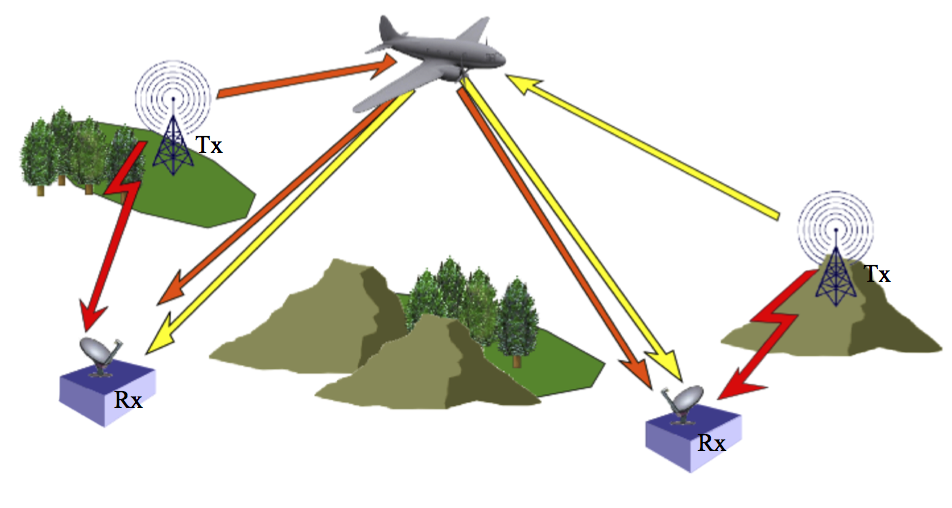
\includegraphics{./figs/CR_1}
  \caption{Depicting a Multistatic Radar}\label{fig:CR_1}
\end{figure}


A bistatic radar uses antennas for transmission and reception at sufficiently different locations that the angles or ranges to the target are significantly different \cite{stand}.

A Commensal Radar (CR) relies on pre-existing transmitter infrastructure to illuminate the target while the receiver receives the scattered energy. These illuminators of opportunity are usually non-cooperative transmitters such as:

\begin{itemize}
\item FM radio
\item DAB 
\item DVB 
\item GSM 
\item Satellite 
\end{itemize}


Some top-level characteristic of CR are listed: 

\begin{itemize}
\item Commensal radars do not need RF spectrum allocation
\item Discovery of the CR receiver is difficult
\item High resistance to Electronic Countermeasures
\item Spatial and frequency diversity possible
\item Possible enhanced RCS at some geometries,
\item Forward Scatter
\item Illumination tilted-downwards for better for low-altitude surveillance
\item Depending on illuminator, range resolution can be fine (DVB) or coarse (FM)
\item Detection capabilities not well defined
\item CR Rx can be made mobile and rapidly deployable to conform to tactics such as frequent sensor relocation to deny enemy fixed targeting
\item CRs easier to replace than expensive air-defence systems


\end{itemize}


\section{CR Literature Review}

This review provides an overview of some important literature relating to CR. In recent years there has been a huge increase in CR-related publications in journals and conferences. The majority of recent publications pertain to algorithmic refinements of CR processing. 

Whilst the amount of CR-related publications has grown in recent years, there are very few publications in the open literature that focus on ECM applied to CR. Internet searches yield hits that mention various research programmes and suggestions for ECM against CR, however, there is little material that is of a technical rigour requiring review.

The NATO group SET-164 (led by Daniel W. O'Hagan) has produced a comprehensive report on CR performance, particularly with regards to clutter modelling. The SET-164 report has been approved for release to Switzerland in 2014.

At least one NATO group, SCI-190 \textit{Electronic Countermeasures to Radar with High-Resolution and Extended Coherent Processing}, has studied countermeasure against CR. SCI-190 was not exclusively focused on ECM against CR, but it formed part of their remit. The SCI-190 group comprised ECM experts from Europe and the US. The group was led Dietmar Mattes of Fraunhofer FHR. The present author attended one SCI-190 meetings and delivered a briefing on CR. The informal consensus amongst the SCI-190 grouping was that ECM applied to CR is ``not easy''.

The review for this report provides an overview of some influential bistatic radar experiments using illuminators of opportunity.  Beginning with a brief discussion of potential illuminators, and the criteria that each should satisfy before being considered 'desirable' for a particular application, there follows a more in-depth assessment of experiments involving these illuminators.  

There are numerous illuminators of opportunity that can potentially be utilised, with some having more desirable radar characteristics than others.  They include: HF radio signals, VHF FM radio signals, DAB, DVB, GSM, GPS, and satellite broadcast services.  There are several conditions that must be satisfied before an illuminator can be considered 'desirable': (i) The transmit power must be sufficient for the coverage required.  (ii) There should be accord between the modulation bandwidth of the illuminating source and the desired range and Doppler resolution. 

The ambiguity function of the more random-like signals will approach the ideal ``thumbtack'' response. A thumbtack ambiguity response represents an excellent ability to discriminate between targets in both range and Doppler. It is important to note, however, that signals producing thumbtack ambiguity functions have a poor Doppler tolerance and are not well suited for targets that can rapidly accelerate and decelerate.  

In \cite{griffiths1986}, Griffiths and Long used analogue television broadcasts from the Crystal Palace transmitter in South London as the illuminator of opportunity to detect aircraft landing and taking off from Heathrow airport.  The receiver was situated at University College London (UCL), 11.8 km from the transmitter.  The transmitted signal was omni-directional with an ERP of 1 MW and operated on four TV channels between 487.25 and 567.25 MHz, with an individual channel bandwidth of 8 MHz, corresponding to 250 kW/channel. The autocorrelation function of the sync-plus-white waveform inherent to analogue television produced high range sidelobes in the order of 5 dB which obscured targets.  It also provided poor range resolution and severe ambiguities at 9600 m and at multiples thereof.  Griffiths and Long concluded that the analogue television signal was not an ideal illuminator of opportunity since its autocorrelation function exhibited broad peaks at 64 $\mu$s intervals corresponding to the line sync pulses.  

In a later work \cite{howland1999} Howland managed to extract Doppler and bearing information from the echoes of the analogue television video carrier to detect and track aircraft at ranges of up to 260 km.  In this application Howland was not concerned with the modulation of the signal and hence did not experience the ambiguities outlined in \cite{griffiths1986}.  Howland's processing exploited the fact that it is possible to achieve a very accurate measure of target Doppler shift using a stable carrier frequency.  Howland, like Griffiths, had a dual channel receiver, one for the reference and the other for target surveillance.  The baseline distance between the Crystal Palace transmitter and the receiver at Pershore was 150 km.  He constructed a phase interferometer consisting of a pair of Yagi antennas separated by 0.6$\lambda$.  It was found that the mutual coupling between the antennas caused inaccuracies in the bearing measurements and had to be compensated for.  As the receiver was situated beyond the Line-of-Sight (LoS) of the transmitter, the direct path interference was substantially reduced.  Howland reported that aircraft could be tracked to ranges up to 260 km from the receiver and 100 km from the transmitter out into the English Channel.  

Zoeller et al. in \cite{zoeller} described a CR system that utilised commercial FM broadcasts as the illuminating signal.  FM radio signals are attractive due to their copious availability; comparatively high transmit powers, and random (noise-like) features, which mean that their ambiguity function (depending on suitable programme content) can approach the ideal thumbtack response.  Zoeller found that, due to the low carrier frequency of FM broadcasts, the CR receiver must use long processing intervals to obtain good Doppler resolution.  The processing intervals ranged from 0.125 to 0.5 seconds which equated to range-rate (velocity) resolutions from 3 m/s to 12 m/s. However, processing intervals of 1 s or more are typically reported in the literature.  Like the other techniques described, their system consisted of two channels, designated reference and target (surveillance).  Zoeller concluded that proper siting of the system is critical to system performance.  This particular system was located on top of Green Mountain, Alabama, USA and allowed detection of commercial aircraft to about 100 km.

A stage of analogue direct signal cancellation in a CR system is desirable as it places a less stringent requirement on the ADC dynamic range.  The UK BAE Systems Multiband Passive Radar Demonstrator \cite{pollard} employed an analogue canceller for this very reason.  It was designed to be configurable to suppress direct signal contributions from a number of different transmission types including DAB. 

In work reported in 2005, Howland, Maksimiuk and Reitsma \cite{howland2005}, now working for the NATO CIA (NCIA) in The Hague, developed a CR system that utilised an FM transmitter located at Lopik, approximately 50 km from the receiver.  As a result of the shorter baseline, Howland suffered a significant increase in direct signal breakthrough compared with that in his previous work described above and in \cite{howland1999}.  In an attempt at reducing the breakthrough, a null in the antenna cardioid was physically steered in the direction of the transmitter.  Once the direct signal had been adaptively filtered, the data could be processed to search for Doppler-shifted and time-delayed echoes of any targets that may be present. 

The receiver bandwidth in \cite{howland2005} was comparable to that of an individual broadcast station resulting in a range resolution of 2 - 3 km.  The authors claimed that this signal clearly offered ``useful target ranging information''.  Whilst upon initial reading this value of range resolution could be considered inadequate, it is important to note that their system detected and tracked large passenger-jet aircraft to ranges in excess of 150 km from the receiver.  As this was the case, then a range resolution of 1.5 km did indeed offer useful ranging information.

As Howland and others have experienced, the greatest single limitation to CW bistatic radar performance is the presence of the Direct Signal Interference (DSI).  O'Hagan and Colone et al in \cite{ohagan1} discussed further the issues of the DSI.  The authors estimated that the target echo can be as low as 90 dB below the DSI breakthrough.  This situation can be improved if the surveillance antenna is shielded from the DSI \cite{ohagan2}, \cite{ohagan3} and \cite{ohagan4}.

In \cite{ohagan1}, due to the positioning of the antennas, the UCL building also acted as a shield from the direct signal.  This form of physical shielding (using the UCL building) achieved a suppression of about 12 dB. 

Research has been conducted towards looking at the suitability of Global System for Mobile communication (GSM) transmissions for use in CR systems.  The advantage of these is that there are GSM base stations honeycombed across large urban areas.  Although the individual transmit power of a GSM base station is low compared to that of FM radio, typically less than 50 W and with a cell range radius less than 2 km, this may by reconciled by their abundance.  GSM transmissions occupy the 870 - 960 MHz band with linear vertical polarisation.  A single sector GMS antenna has an azimuth beamwidth of 60$^\circ$ and an elevation beamwidth of 16.5$^\circ$.  The length of the antenna sector is 1.5 m and the beam tilt can be set between $\pm$12$^\circ$.  The gain of such elements is 15 dBi \cite{kitchen}.  Tan et al. in \cite{tan} investigated the feasibility of using GSM to detect and track different types of ground moving targets, such as vehicle and human movement.  Unlike FM and analogue TV broadcast signals, where the signal changes as a function of the programme content, the effective bandwidth of a GSM carrier signal is constant.  Tan et al. report a maximum range resolution of 1.845 km with a theoretical carrier bandwidth of 81.3 kHz.  Since the small bandwidths of a GSM carrier signal (81.3 kHz) resulted in a range resolution comparable to that of a single FM channel, it was too poor to discriminate between the human and vehicle targets. However, Tan demonstrated results for the Doppler tracking of cooperative ground-moving targets (i.e. a small truck and a human).

In separate work Poullin \cite{poullin} investigated CR based on digital broadcast signals (DAB, DVB) with Coded Orthogonal Frequency Division Multiplexing (COFDM) modulation.  

It is often the case that weak target echoes at far ranges are masked by stronger echoes from closer-in targets.  This masking effect is due to the high peak-sidelobe level of the ambiguity function and cannot be removed by conventional Moving Target Indicator (MTI) techniques because of the extensive range-Doppler spreading of the interference.  The situation is well covered by Kulpa and Czekala in \cite{kulpa1} and by Colone and O'Hagan et al. in \cite{ohagan5}.  In \cite{kulpa1}, strong multipath and target echoes are progressively cancelled (whilst retaining in memory the location of the strong targets).  However in \cite{ohagan5}, a multistage processing algorithm was developed for disturbance cancellation and target detection based on projections of the received signals in a subspace orthogonal to both the disturbance and previously detected targets.  The technique dealt with the interference spreading in the Doppler dimension by processing the data in short batches and later recombining each batch. This permitted a wider cancellation notch in the Doppler domain thus yielding an improved removal of the disturbance together with a reduced computational load.  Unlike Kulpa's and Czekala's technique, the cancellation method in \cite{ohagan5} has been tested and operates well on real FM data, thus extending the detection range of the passive radar.

In around 2005, one of the very few commercially available CRs was the Lockheed Martin Silent Sentry system that utilised FM radio broadcast transmissions.  Silent Sentry could be deployed on a fixed or a mobile (vehicle) platform.  The radar use a vertically polarised circular array antenna, which was 1.5 m tall and comprised eight dipoles arranged evenly on a 1 m diameter cylinder.  The final iteration the radar had the dipoles arranged on a 2 m diameter circle for generating narrower and higher gain beams, thus providing greater range and higher accuracy.  Tests have shown that the sidelobe levels were sufficiently high that they impeded target tracking.  However, modifications to the antenna, such as the addition of parasitic elements to uniformly increase the bandwidth over the FM band and compensating for mutual coupling, were expected to achieve a PSLR of around 30 dB.  Another antenna option was available in the form of a horizontally polarised linear array of dipoles for extended range sector coverage.  The linear array was deployed for longer range applications (200 km).  Silent Sentry 3 version 2 (SS3v2) provided four times the processing capability over its earlier iteration, SS3v1.  It had ten RF input channels providing the potential for greater system flexibility for the addition of extra antennas, or for continuously monitoring the signal environment.  The latter case is particularly useful for accurately predicting the propagation conditions.  The Lockheed Martin engineers have found that they occasionally experience ducting, which is an inversion in the thermal layer that results in propagation anomalies, so a signal monitoring channel could provide intelligence about possible environmental anomalies \cite{lockheed}.

BAE Systems and Roke Manor Research created the CELLphone raDAR (CELLDAR) system. CELLDAR utilised transmission from GSM 900, 1800 and 1900 mobile phone broadcasts and operated in a multistatic radar configuration. The system was intended for the detection and tracking of moving air, land and sea-based objects \cite{celldar}.  The system suffers significantly from interference from cars, thus limiting detection performance \cite{rickett}.  To improve and enhance system performance, CELLDAR also encompassed acoustic sensors (translates the Doppler frequency into the audio band) to 'hear' emissions from the target. The present programme status of CELLDAR is not known, but it is likely that the project has ceased.

Despite the commercial failure of Silent Sentry and CELLDAR, several other organisations with long traditions in radar have CR Research and Development programmes. Some of these, including Thales, Airbus, and Selex currently offer (or are soon to offer) CR as commercial products. Thales with their Homeland Alerter (HA-100) and Airbus (formerly Cassidian) with their Passive Radar have been leading the commercial drive for CR technology.

The HA-100 is relies on FM illuminators whilst the Airbus Passive Radar employs a multiband approach encompassing FM, DAB and DVB. Both systems have developed rapidly over the past five years. Their performance improvements have been impressive with significant refinements to system hardware and signal processing. Both Thales and Airbus have developed advances Mission Planning Tools, antenna array beamforming and null-steering, robust interference suppression techniques.

Fraunhofer FHR is not a commercial enterprise but it collaborates closely with Airbus and Thales. FHR itself has focused primarily on DAB and DVB based CRs and has developed a number of demonstrator systems including DELIA (DAB), SANDY (DAB), CoRa (DAB and DVB), and CoRa-11 (11-element array DVB CR).

The German and French Ministries of Defence are enthusiastic about CR technology and are keen for CR to form part of the air-defence infrastructure.  In the civilian context, CR is also being seriously considered as a supplementary technology for Air Traffic Management (ATM).

According to \cite{caa_1}, the UK Civil Aviation Authority (CAA) strategy with regards to CR can be summarised as:

\begin{itemize}
\item Future ATM capability based on combination of independent ground-based surveillance and airborne derived down-linked data, driven by performance requirements and new technology.

\item Still be a requirement for PSR coverage by primary radar due to national defence and system security needs. Primary radar will be used as a back-up system and as a means of tracking non-cooperative users. 

\item Multi-static PSR is a replacement for the current primary radar solution that is more cost-effective and reduces spectrum requirements. Further proof of concept work is required before multi-static PSR is accepted as a primary surveillance means.

\item A CAA roadmap for implementation of changes to surveillance over the next 20 years plans the ``introduction of Multi-Static PSR to replace primary radar'' in 2015 to 2020.

\item Beyond 2020, the CAA plan a ``Wider roll out of Multi-Static PSR''.
 
\end{itemize}

The ERA Company in the Czech Republic are currently developing an Passive Emitter Tracker (PET) and CR dual operation system. Likewise, a consortium in Poland including Warsaw University of Technology, the Ministry of Defence and radar industry are also developing a PET-CR system, which is intended to be at TRL-9 upon project completion.

 